\documentclass{scrartcl}
\usepackage[latin1]{inputenc}
\usepackage[T1]{fontenc}
\usepackage[ngerman]{babel}
\usepackage{amsmath}
\usepackage{amssymb}
\usepackage{icomma}
%\usepackage[dvips]{graphicx}
%\usepackage{floatflt}
%\usepackage{enumitem}
%\usepackage{babel}
\usepackage{blindtext}
%\usepackage{showframe}
\usepackage{calc}
\usepackage{wrapfig}
\def\BILD{\rule{0.4\textwidth}{4cm}}

\usepackage{graphicx}
\usepackage{placeins}
\usepackage{multirow}
\usepackage{subfig}
\usepackage{url}

\renewcommand{\topfraction}{.85}
\renewcommand{\bottomfraction}{.7}
\renewcommand{\textfraction}{.15}
\renewcommand{\floatpagefraction}{.66}
\renewcommand{\dbltopfraction}{.66}
\renewcommand{\dblfloatpagefraction}{.66}
\setcounter{topnumber}{9}
\setcounter{bottomnumber}{9}
\setcounter{totalnumber}{20}
\setcounter{dbltopnumber}{9}
\setlength{\intextsep}{0cm plus1cm minus1cm}
\pdfminorversion = 5
\usepackage{setspace}
\onehalfspacing

\begin{document}
\title{Versuch 2: Polarisiertes Licht}


\date{27.11.2010}


\author{Gruppe 5a: Gia-Danh Lam, Nils Haldenwang}

\maketitle
\tableofcontents

\section{Einleitung}


\section{Aufgaben}
\begin{tabular}{lp{12cm}}
(a)& Beschreibung der Erzeugung von linear polarisiertem Licht mit doppelbrechenden Kristallen:
Anisotrope Kristalle haben die Eigenschaft, das einfallende Licht je nach Polarisation und Einfall unterschiedlich zu brechen. Dieses Ph�nomen kann man mithilfe von optischen Achsen erkl�ren. Die optische Achse kann man sich als eine schr�ge Fl�che innerhalb des Materials vorstellen, die das Licht nochmals brechen kann. Wenn die Auslenkung der elektromagnetischen Welle senkrecht zur optischen Achse ausgerichtet ist, wird das Licht nach dem Snelliusschem Brechungsgesetz gebrochen. Diesen Strahl nennt man ordentlichen Strahl. Wenn die Auslenkung aber anders ist, kann man die elektromagnetische Welle als �berlagerung von zwei Wellen auffassen, wobei einer von ihnen nicht senkrecht zur optischen Achse schwingt. Dieser Strahl  wird als au�erordentlicher Strahl bezeichnet. Da die Auslenkung hier nicht parallel zur optischen Achse ist, wird dieser Strahl mit einem anderem Brechungsindex gebrochen. Dadurch wird aus ehemals einem Strahl zwei Strahlen mit genau senkrecht zueinander ausgerichteten Auslenkung, d.h. zwei linear polarisierte Strahlen. \\
(b)& Das Nicolsche Prisma ist ein Polarisationsprisma. \\
\end{tabular}
\begin{figure}[htb!]
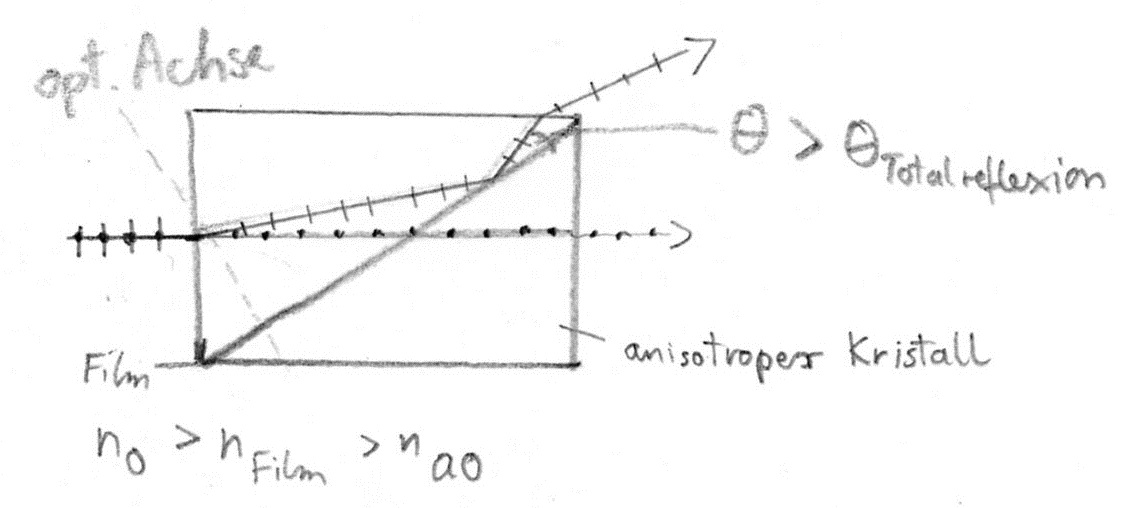
\includegraphics[width=\columnwidth]{pics/nprisma}%
\caption{Skizze f�r ein Polarisationsprisma}%
\label{fig:nprisma}%
\end{figure}

\subsection{Erzeugung und Analyse von polarisiertem Licht} 
\subsubsection{Vorversuche}
Es soll zun�chst das Malus-Gesetz �berpr�ft werden, das lautet:
\begin{equation}
I=I_0 \cdot cos^2(\alpha)
\label{eq:1}
\end{equation}
Dazu haben wir die Intensit�t I von linear polarisiertem Licht bei verschiedenen Stellungen $(\alpha)$ des Polarisators gemessen. Das linear polarisierte Licht sollte am Anfang parallel zur Ausrichtung des Polarisators schwingen, also bei der Einstellung von 0�. Uns ist bei sp�teren Versuchen aufgefallen, dass der im Versuch angegebene Winkel $\alpha$ nicht ganz stimmt, sondern um ca. 3� verschoben ist.
\begin{table}[htb!]
\begin{tabular}{l|r|r|r|r|r|r|r|r|r|r|}
\hline
$\alpha$ in �& 0&10&20&30&40&50&60&70&80&90\\
\hline
gem.Intensit�t I&117&111&99&82&62,2&42,3&24,6&10,2&2,4&1,8\\
\hline
berechn. I &117&113,5&103,3&87,8&68,7&48,3&29,3&13,7&3,5&0\\
\hline
korr. $\alpha$ in �& 3&13&23&33&43&53&63&73&83&93\\
\hline
berechn. I&117&111,4&99,4&82,5&62,8&42,5&24,2&10,0&1,7&0,3\\
\end{tabular}
\caption{}
\label{tab: mgesetz}
\end{table}



 
\end{document}



